\section{Methods}
\label{sec:methods}
\begin{figure*}[t]
\centering
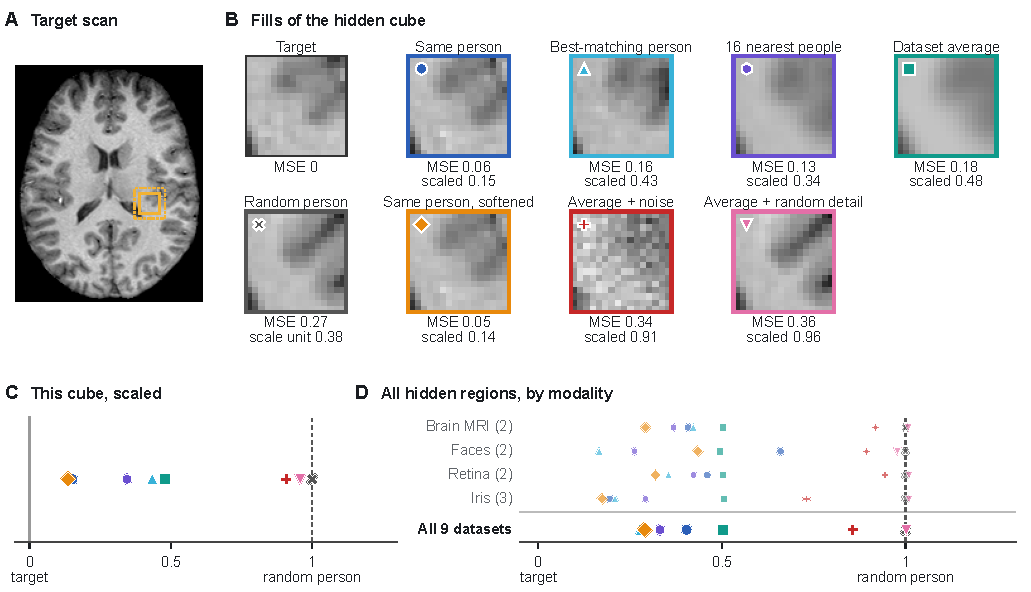
\includegraphics[width=0.86\textwidth]{fig/fig_explainer_mse_v3.pdf}
\caption{\textbf{How one row of Figure~\ref{fig:summary} is computed: \acs{MSE} on one brain cube.}
\textbf{A,} One QTIM brain scan; solid square: the hidden 16\,mm cube; dashed square: the 4\,mm ring of visible context around it.
\textbf{B,} The target cube and each fill, framed in its color and marker from Figure~\ref{fig:summary} (Section~\ref{sec:controls}): the same person's second scan; the best-matching person, the unrelated person whose cube is most like the target's (found by looking inside the hidden cube); the average of the 16 unrelated people with the most similar visible ring; the dataset average of all unrelated people; one random person; and three controls: the second scan with 85\% of its detail kept (softened), the average plus white noise, and the average plus a random person's detail, each at the same strength.
Below each fill: its \acs{MSE} to the target and that \acs{MSE} scaled by the average \acs{MSE} of 16 random people (0.38), so that 0 is the target and 1 is a random person.
\textbf{C,} The same cube on this scale.
\textbf{D,} Faint rows: means over all hidden regions and datasets of one modality (number of datasets in brackets); bold row: mean over the nine datasets, which is the \acs{MSE} row of Figure~\ref{fig:summary}.
PAPILA and IXI have no second image, so their same-person infill is the mirrored image of the other side.
The cube was chosen before drawing as the one of 1{,}472 complete cubes closest to the QTIM averages; brain values are provisional.
Even on one cube, \acs{MSE} scores the softened same person (0.14) as close as the same person (0.15) and puts the dataset average (0.48) at half a random person.}
\label{fig:explainer}
\end{figure*}
% Sources: make_fig_explainer_v3.py output (v1 figure kept as fig/fig_explainer_mse.pdf); results/donor_ladder_brain_metrics.json
% (lambda_shrink); results/cross_modality/common_all.json and fig_metric_summary_R.json (panel D).


\subsection{Terms and fills}
\label{sec:ladder}
\label{sec:controls}
The \emph{target} is the region of a person's image hidden from the inpainting model: a 16\,mm cube in the brain, a square window in the 2D images.
The \emph{context ring} is a band of visible pixels around it (4\,mm in the brain).
A \emph{fill} is any content placed into the hidden region and compared with the target; every fill here is a real image, an average of real images, or a control built from them, and no generative model is evaluated.
\emph{Valid pixels} are pixels observed in both target and fill (field of view, brain mask, iris without lids and reflections); other pixels are missing, never zero.
\emph{Unrelated people} are everyone outside the target person's family.

The \emph{true person} is the same region in a second image of the same person (second \ac{MRI} session, photograph, visit or capture of the same eye); where a dataset has none (PAPILA, IXI), the opposite side takes its place in cross-dataset summaries.
The \emph{opposite side} is the mirrored region of the other hemisphere, half face or eye; a \emph{sibling} is a recorded family member.
A \emph{stranger} is one random unrelated person, and we draw 16 per target.
The \emph{dataset mean} averages all unrelated people at each pixel, using only people valid there.
\emph{Look-alikes} are chosen from the context only: we rank unrelated people by the mean squared difference between their context ring and the target's ring and average the hidden region of the 16 closest (\emph{mean of 16 look-alikes}).
The \emph{oracle look-alike} is instead the one unrelated person whose hidden region is closest to the target; it uses the answer and is an upper bound.

With $\hat\mu$ the dataset mean and $f$ the true person's second image, the \emph{shrunk true person} is $\hat\mu+\lambda(f-\hat\mu)$: nothing is cropped, the individual detail $f-\hat\mu$ is scaled down.
We set $\lambda=1-\bar Q/2$, the fraction of individual detail a second image keeps on average ($\bar Q$ from Eq.~\ref{eq:unit}; $\lambda=0.85$ for QTIM), which mimics what squared-error training produces under uncertainty.
\emph{Wrong detail} is $\hat\mu$ plus a stranger's individual detail made orthogonal to the target's and rescaled to the same norm; \emph{noise} is $\hat\mu$ plus white noise with the standard deviation of the target's individual detail.

\subsection{Distances and scales}
For target $x_i$ and fill $f$ on valid pixels $E_i$,
\begin{equation}
e_i(f)=\frac{1}{|E_i|}\sum_{v\in E_i}\bigl(x_i(v)-f(v)\bigr)^2,\quad
Q(f)=\frac{\sum_i e_i(f)}{\sum_i e_i(\hat\mu)},
\label{eq:unit}
\end{equation}
where $v$ is a pixel and $i$ runs over all targets and regions; summing before dividing avoids unstable per-target ratios.
The dataset mean has $Q=1$, and if a person is the mean plus independent detail, a stranger has $Q\approx2$.
For all metrics we also use a stranger scale,
\begin{equation}
R(f)=\frac{\bar d(f)-\bar d_0}{\bar d(\mathrm{strangers})-\bar d_0},
\label{eq:anchors}
\end{equation}
with $d$ the metric written as a distance (similarities negated), $\bar d$ its average over targets and regions, $\bar d(\mathrm{strangers})$ the average over the 16 random strangers and $\bar d_0$ the distance of the target to itself, so $R=0$ is the target and $R=1$ a typical stranger (Figure~\ref{fig:explainer}).
The stranger is the natural unit because it is the fill a model produces when it ignores the context and copies an arbitrary training image, and because every metric can measure it on every dataset; a metric that cannot place the true person below 1 does not see the person at all.
The brain table also anchors $\bar d_0$ on the second scan, because two sessions of one brain differ.

\subsection{Metrics, uncertainty and status}
We compute ten variants in four families.
\emph{Error and similarity}: \ac{MSE}, \ac{SSIM} and three tolerance scores from protein-structure comparison, \ac{TM}-like~\cite{tmscore2004}, \ac{GDT}-like~\cite{zemla2003lga} and \ac{lDDT}-like~\cite{lddt2013}, which count positions that agree within a tolerance (fixed, or the typical difference between two scans of one person) so that a few large differences cannot dominate.
\emph{\acs{LPIPS}} with AlexNet and VGG features~\cite{zhang2018lpips}.
\emph{Topology}: Betti matching~\cite{betti2023} and persistence diagrams of thresholded images.
\emph{Set level}: \ac{FID}~\cite{heusel2017fid} and \ac{FWD}~\cite{fwd2025}, which compare the distribution of all fills of a rung with that of all targets.
Kernels and tolerances are in the supplement.
Intervals are 95\% bootstrap intervals (2{,}000 resamples of people or families).
One-sided tests ask whether the second image beats the dataset mean (T1), the shrunk true person (T2), wrong detail (T3a) and noise (T3b), Holm-corrected within dataset.
\statusfinal\ marks results whose preprocessing passed visual \ac{QC}; \statuspre\ marks provisional ones.
Maps use Gaussian local averages with standard deviation $w/\sqrt{12}$ for window width $w$.

\subsection{Datasets}
\label{sec:m-brain}
\label{sec:m-fundus}
\label{sec:m-face}
\label{sec:m-iris}
Table~\ref{tab:datasets} lists the nine image sets.
Brain: QTIM~\cite{qtim2026,strike2019} (twins and siblings, 23 with a second session) and IXI~\cite{ixi} (100 scans across three sites), corrected for slow intensity variation (N4), affinely aligned to the symmetric \ac{MNI} template and standardized within the brain mask; 32 random cubes, both hemispheres.
Retina: GRAPE~\cite{grape2023} (both eyes, repeated visits) and PAPILA~\cite{papila2022} (both eyes), left eyes mirrored, optic-disc frame, green channel at 128 pixels.
Faces: CelebA~\cite{celeba2015} and IMDb-WIKI~\cite{rothe2018}, landmark-aligned and pose-restricted; the opposite side is the mirrored other half of the face, with a midline band excluded.
Irises: UTIRIS~\cite{hosseini2010} (\ac{NIR} and \ac{VIS}) and UPOL~\cite{dobes2004}, segmented and unwrapped into strips with lid and reflection masks.
Brain, retina and iris remain provisional until registration and mask \ac{QC} are complete.

\begin{table}[t]
\centering
\caption{\textbf{Datasets and where their ladders sit} ($Q$, Eq.~\ref{eq:unit}: 1 = dataset mean, about 2 = stranger; n/a = no such image; look-alike = one context-selected person).
The stranger is near 2 everywhere; the second image is the closest rung except in faces, where pose and lighting change between photographs.}
\label{tab:datasets}
\scriptsize
\setlength{\tabcolsep}{2.2pt}
\begin{tabular}{@{}lrrrrrr@{}}
\toprule
Dataset & Persons & Targets & 2nd img & Opp. side & Look-alike & Stranger \\
\midrule
% Generated from tab/dataset_card.tex by a column subset; do not edit by hand.
QTIM\statuspre & 168 fam. & 221 & 0.30 & 1.51 & 1.18 & 1.99 \\
CelebA\statusfinal & 921 & 921 & 1.28 & 0.95 & 0.80 & 2.02 \\
IMDb-WIKI\statusfinal & 453 fam. & 678 & 1.39 & 1.06 & 0.80 & 2.02 \\
GRAPE\statuspre & 134 & 239 & 0.39 & 1.31 & 1.08 & 1.99 \\
PAPILA\statuspre & 244 & 488 & $\cdot$ & 1.44 & 1.32 & 1.99 \\
UTIRIS NIR\statuspre & 78 & 156 & 0.40 & 1.21 & 0.58 & 1.98 \\
UTIRIS VIS\statuspre & 79 & 158 & 0.57 & 1.29 & 0.85 & 1.98 \\
UPOL\statuspre & 64 & 128 & 0.18 & 1.12 & 0.84 & 1.96 \\
IXI\statuspre & 100 & 100 & $\cdot$ & 1.31 & 1.02 & 1.98 \\
\bottomrule

\end{tabular}
\end{table}
